\documentclass[1p]{elsarticle_modified}
%\bibliographystyle{elsarticle-num}

%\usepackage[colorlinks]{hyperref}
%\usepackage{abbrmath_seonhwa} %\Abb, \Ascr, \Acal ,\Abf, \Afrak
\usepackage{amsfonts}
\usepackage{amssymb}
\usepackage{amsmath}
\usepackage{amsthm}
\usepackage{scalefnt}
\usepackage{amsbsy}
\usepackage{kotex}
\usepackage{caption}
\usepackage{subfig}
\usepackage{color}
\usepackage{graphicx}
\usepackage{xcolor} %% white, black, red, green, blue, cyan, magenta, yellow
\usepackage{float}
\usepackage{setspace}
\usepackage{hyperref}

\usepackage{tikz}
\usetikzlibrary{arrows}

\usepackage{multirow}
\usepackage{array} % fixed length table
\usepackage{hhline}

%%%%%%%%%%%%%%%%%%%%%
\makeatletter
\renewcommand*\env@matrix[1][\arraystretch]{%
	\edef\arraystretch{#1}%
	\hskip -\arraycolsep
	\let\@ifnextchar\new@ifnextchar
	\array{*\c@MaxMatrixCols c}}
\makeatother %https://tex.stackexchange.com/questions/14071/how-can-i-increase-the-line-spacing-in-a-matrix
%%%%%%%%%%%%%%%

\usepackage[normalem]{ulem}

\newcommand{\msout}[1]{\ifmmode\text{\sout{\ensuremath{#1}}}\else\sout{#1}\fi}
%SOURCE: \msout is \stkout macro in https://tex.stackexchange.com/questions/20609/strikeout-in-math-mode

\newcommand{\cancel}[1]{
	\ifmmode
	{\color{red}\msout{#1}}
	\else
	{\color{red}\sout{#1}}
	\fi
}

\newcommand{\add}[1]{
	{\color{blue}\uwave{#1}}
}

\newcommand{\replace}[2]{
	\ifmmode
	{\color{red}\msout{#1}}{\color{blue}\uwave{#2}}
	\else
	{\color{red}\sout{#1}}{\color{blue}\uwave{#2}}
	\fi
}

\newcommand{\Sol}{\mathcal{S}} %segment
\newcommand{\D}{D} %diagram
\newcommand{\A}{\mathcal{A}} %arc


%%%%%%%%%%%%%%%%%%%%%%%%%%%%%5 test

\def\sl{\operatorname{\textup{SL}}(2,\Cbb)}
\def\psl{\operatorname{\textup{PSL}}(2,\Cbb)}
\def\quan{\mkern 1mu \triangleright \mkern 1mu}

\theoremstyle{definition}
\newtheorem{thm}{Theorem}[section]
\newtheorem{prop}[thm]{Proposition}
\newtheorem{lem}[thm]{Lemma}
\newtheorem{ques}[thm]{Question}
\newtheorem{cor}[thm]{Corollary}
\newtheorem{defn}[thm]{Definition}
\newtheorem{exam}[thm]{Example}
\newtheorem{rmk}[thm]{Remark}
\newtheorem{alg}[thm]{Algorithm}

\newcommand{\I}{\sqrt{-1}}
\begin{document}

%\begin{frontmatter}
%
%\title{Boundary parabolic representations of knots up to 8 crossings}
%
%%% Group authors per affiliation:
%\author{Yunhi Cho} 
%\address{Department of Mathematics, University of Seoul, Seoul, Korea}
%\ead{yhcho@uos.ac.kr}
%
%
%\author{Seonhwa Kim} %\fnref{s_kim}}
%\address{Center for Geometry and Physics, Institute for Basic Science, Pohang, 37673, Korea}
%\ead{ryeona17@ibs.re.kr}
%
%\author{Hyuk Kim}
%\address{Department of Mathematical Sciences, Seoul National University, Seoul 08826, Korea}
%\ead{hyukkim@snu.ac.kr}
%
%\author{Seokbeom Yoon}
%\address{Department of Mathematical Sciences, Seoul National University, Seoul, 08826,  Korea}
%\ead{sbyoon15@snu.ac.kr}
%
%\begin{abstract}
%We find all boundary parabolic representation of knots up to 8 crossings.
%
%\end{abstract}
%\begin{keyword}
%    \MSC[2010] 57M25 
%\end{keyword}
%
%\end{frontmatter}

%\linenumbers
%\tableofcontents
%
\newcommand\colored[1]{\textcolor{white}{\rule[-0.35ex]{0.8em}{1.4ex}}\kern-0.8em\color{red} #1}%
%\newcommand\colored[1]{\textcolor{white}{ #1}\kern-2.17ex	\textcolor{white}{ #1}\kern-1.81ex	\textcolor{white}{ #1}\kern-2.15ex\color{red}#1	}

{\Large $\underline{11a_{250}~(K11a_{250})}$}

\setlength{\tabcolsep}{10pt}
\renewcommand{\arraystretch}{1.6}
\vspace{1cm}\begin{tabular}{m{100pt}>{\centering\arraybackslash}m{274pt}}
\multirow{5}{120pt}{
	\centering
	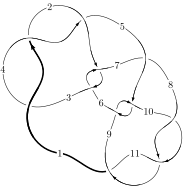
\includegraphics[width=112pt]{../../../GIT/diagram.site/Diagrams/png/499_11a_250.png}\\
\ \ \ A knot diagram\footnotemark}&
\allowdisplaybreaks
\textbf{Linearized knot diagam} \\
\cline{2-2}
 &
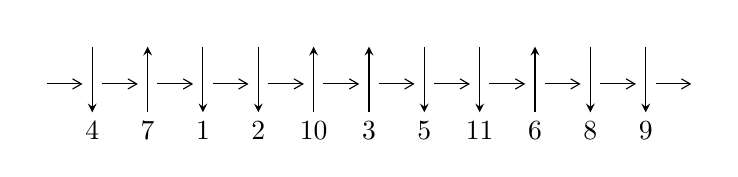
\begin{tikzpicture}[x=20pt, y=17pt]
	% nodes
	\node (C0) at (0, 0) {};
	\node (C1) at (1, 0) {};
	\node (C1U) at (1, +1) {};
	\node (C1D) at (1, -1) {4};

	\node (C2) at (2, 0) {};
	\node (C2U) at (2, +1) {};
	\node (C2D) at (2, -1) {7};

	\node (C3) at (3, 0) {};
	\node (C3U) at (3, +1) {};
	\node (C3D) at (3, -1) {1};

	\node (C4) at (4, 0) {};
	\node (C4U) at (4, +1) {};
	\node (C4D) at (4, -1) {2};

	\node (C5) at (5, 0) {};
	\node (C5U) at (5, +1) {};
	\node (C5D) at (5, -1) {10};

	\node (C6) at (6, 0) {};
	\node (C6U) at (6, +1) {};
	\node (C6D) at (6, -1) {3};

	\node (C7) at (7, 0) {};
	\node (C7U) at (7, +1) {};
	\node (C7D) at (7, -1) {5};

	\node (C8) at (8, 0) {};
	\node (C8U) at (8, +1) {};
	\node (C8D) at (8, -1) {11};

	\node (C9) at (9, 0) {};
	\node (C9U) at (9, +1) {};
	\node (C9D) at (9, -1) {6};

	\node (C10) at (10, 0) {};
	\node (C10U) at (10, +1) {};
	\node (C10D) at (10, -1) {8};

	\node (C11) at (11, 0) {};
	\node (C11U) at (11, +1) {};
	\node (C11D) at (11, -1) {9};
	\node (C12) at (12, 0) {};

	% arrows
	\draw[->,>={angle 60}]
	(C0) edge (C1) (C1) edge (C2) (C2) edge (C3) (C3) edge (C4) (C4) edge (C5) (C5) edge (C6) (C6) edge (C7) (C7) edge (C8) (C8) edge (C9) (C9) edge (C10) (C10) edge (C11) (C11) edge (C12) ;	\draw[->,>=stealth]
	(C1U) edge (C1D) (C2D) edge (C2U) (C3U) edge (C3D) (C4U) edge (C4D) (C5D) edge (C5U) (C6D) edge (C6U) (C7U) edge (C7D) (C8U) edge (C8D) (C9D) edge (C9U) (C10U) edge (C10D) (C11U) edge (C11D) ;
	\end{tikzpicture} \\
\hhline{~~} \\& 
\textbf{Solving Sequence} \\ \cline{2-2} 
 &
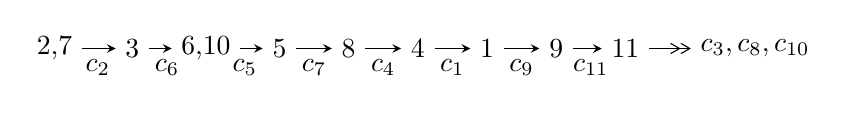
\begin{tikzpicture}[x=25pt, y=7pt]
	% node
	\node (A0) at (-1/8, 0) {2,7};
	\node (A1) at (1, 0) {3};
	\node (A2) at (33/16, 0) {6,10};
	\node (A3) at (25/8, 0) {5};
	\node (A4) at (33/8, 0) {8};
	\node (A5) at (41/8, 0) {4};
	\node (A6) at (49/8, 0) {1};
	\node (A7) at (57/8, 0) {9};
	\node (A8) at (65/8, 0) {11};
	\node (C1) at (1/2, -1) {$c_{2}$};
	\node (C2) at (3/2, -1) {$c_{6}$};
	\node (C3) at (21/8, -1) {$c_{5}$};
	\node (C4) at (29/8, -1) {$c_{7}$};
	\node (C5) at (37/8, -1) {$c_{4}$};
	\node (C6) at (45/8, -1) {$c_{1}$};
	\node (C7) at (53/8, -1) {$c_{9}$};
	\node (C8) at (61/8, -1) {$c_{11}$};
	\node (A9) at (10, 0) {$c_{3},c_{8},c_{10}$};

	% edge
	\draw[->,>=stealth]	
	(A0) edge (A1) (A1) edge (A2) (A2) edge (A3) (A3) edge (A4) (A4) edge (A5) (A5) edge (A6) (A6) edge (A7) (A7) edge (A8) ;
	\draw[->>,>={angle 60}]	
	(A8) edge (A9);
\end{tikzpicture} \\ 

\end{tabular} \\

\footnotetext{
The image of knot diagram is generated by the software ``\textbf{Draw programme}" developed by Andrew Bartholomew(\url{http://www.layer8.co.uk/maths/draw/index.htm\#Running-draw}), where we modified some parts for our purpose(\url{https://github.com/CATsTAILs/LinksPainter}).
}\phantom \\ \newline 
\centering \textbf{Ideals for irreducible components\footnotemark of $X_{\text{par}}$} 
 
\begin{align*}
I^u_{1}&=\langle 
15 u^9-5 u^8+43 u^7-48 u^6+65 u^5-93 u^4+16 u^3-58 u^2+11 b-11 u-34,\\
\phantom{I^u_{1}}&\phantom{= \langle  }-8 u^9- u^8-31 u^7+19 u^6-42 u^5+65 u^4-10 u^3+61 u^2+11 a+22 u+24,\\
\phantom{I^u_{1}}&\phantom{= \langle  }u^{10}+3 u^8-2 u^7+4 u^6-5 u^5- u^4-4 u^3-3 u^2-3 u-1\rangle \\
I^u_{2}&=\langle 
-3.80757\times10^{52} u^{41}-8.35941\times10^{52} u^{40}+\cdots+3.13757\times10^{53} b-1.31429\times10^{54},\\
\phantom{I^u_{2}}&\phantom{= \langle  }4.68086\times10^{52} u^{41}+1.61851\times10^{53} u^{40}+\cdots+6.27515\times10^{53} a+2.05544\times10^{54},\\
\phantom{I^u_{2}}&\phantom{= \langle  }u^{42}+2 u^{41}+\cdots+160 u-32\rangle \\
I^u_{3}&=\langle 
- u^4+u^3-2 u^2+b-1,\;u^4- u^3+2 u^2+a- u+1,\;u^5- u^4+2 u^3- u^2+u-1\rangle \\
\\
I^v_{1}&=\langle 
a,\;v^4+2 v^3+v^2+b-2 v-1,\;v^5+3 v^4+4 v^3+v^2- v-1\rangle \\
\end{align*}
\raggedright * 4 irreducible components of $\dim_{\mathbb{C}}=0$, with total 62 representations.\\
\footnotetext{All coefficients of polynomials are rational numbers. But the coefficients are sometimes approximated in decimal forms when there is not enough margin.}
\newpage
\renewcommand{\arraystretch}{1}
\centering \section*{I. $I^u_{1}= \langle 15 u^9-5 u^8+\cdots+11 b-34,\;-8 u^9- u^8+\cdots+11 a+24,\;u^{10}+3 u^8+\cdots-3 u-1 \rangle$}
\flushleft \textbf{(i) Arc colorings}\\
\begin{tabular}{m{7pt} m{180pt} m{7pt} m{180pt} }
\flushright $a_{2}=$&$\begin{pmatrix}1\\0\end{pmatrix}$ \\
\flushright $a_{7}=$&$\begin{pmatrix}0\\u\end{pmatrix}$ \\
\flushright $a_{3}=$&$\begin{pmatrix}1\\- u^2\end{pmatrix}$ \\
\flushright $a_{6}=$&$\begin{pmatrix}- u\\u^3+u\end{pmatrix}$ \\
\flushright $a_{10}=$&$\begin{pmatrix}\frac{8}{11} u^9+\frac{1}{11} u^8+\cdots-2 u-\frac{24}{11}\\-\frac{15}{11} u^9+\frac{5}{11} u^8+\cdots+u+\frac{34}{11}\end{pmatrix}$ \\
\flushright $a_{5}=$&$\begin{pmatrix}-\frac{1}{11} u^9-\frac{7}{11} u^8+\cdots- u-\frac{8}{11}\\-\frac{5}{11} u^9-\frac{2}{11} u^8+\cdots+2 u+\frac{15}{11}\end{pmatrix}$ \\
\flushright $a_{8}=$&$\begin{pmatrix}\frac{3}{11} u^9+\frac{10}{11} u^8+\cdots-3 u-\frac{9}{11}\\-\frac{1}{11} u^9+\frac{4}{11} u^8+\cdots- u-\frac{8}{11}\end{pmatrix}$ \\
\flushright $a_{4}=$&$\begin{pmatrix}-\frac{6}{11} u^9-\frac{9}{11} u^8+\cdots+u+\frac{7}{11}\\-\frac{5}{11} u^9-\frac{2}{11} u^8+\cdots+2 u+\frac{15}{11}\end{pmatrix}$ \\
\flushright $a_{1}=$&$\begin{pmatrix}-\frac{6}{11} u^9-\frac{9}{11} u^8+\cdots+u+\frac{7}{11}\\\frac{2}{11} u^9-\frac{8}{11} u^8+\cdots+u-\frac{6}{11}\end{pmatrix}$ \\
\flushright $a_{9}=$&$\begin{pmatrix}\frac{8}{11} u^9+\frac{1}{11} u^8+\cdots-2 u-\frac{24}{11}\\-\frac{15}{11} u^9+\frac{5}{11} u^8+\cdots+u+\frac{34}{11}\end{pmatrix}$ \\
\flushright $a_{11}=$&$\begin{pmatrix}\frac{4}{11} u^9-\frac{16}{11} u^8+\cdots+2 u-\frac{12}{11}\\-\frac{8}{11} u^9-\frac{1}{11} u^8+\cdots+3 u+\frac{35}{11}\end{pmatrix}$\\ \flushright $a_{11}=$&$\begin{pmatrix}\frac{4}{11} u^9-\frac{16}{11} u^8+\cdots+2 u-\frac{12}{11}\\-\frac{8}{11} u^9-\frac{1}{11} u^8+\cdots+3 u+\frac{35}{11}\end{pmatrix}$\\&\end{tabular}
\flushleft \textbf{(ii) Obstruction class $= -1$}\\~\\
\flushleft \textbf{(iii) Cusp Shapes $= -\frac{148}{11} u^9+\frac{20}{11} u^8-\frac{436}{11} u^7+\frac{368}{11} u^6-\frac{612}{11} u^5+\frac{856}{11} u^4+\frac{24}{11} u^3+\frac{584}{11} u^2+20 u+\frac{290}{11}$}\\~\\
\newpage\renewcommand{\arraystretch}{1}
\flushleft \textbf{(iv) u-Polynomials at the component}\newline \\
\begin{tabular}{m{50pt}|m{274pt}}
Crossings & \hspace{64pt}u-Polynomials at each crossing \\
\hline $$\begin{aligned}c_{1},c_{3},c_{4}\\c_{8},c_{10},c_{11}\end{aligned}$$&$\begin{aligned}
&u^{10}-2 u^9-3 u^8+6 u^7+4 u^6-3 u^5-7 u^4-2 u^3+5 u^2+u+1
\end{aligned}$\\
\hline $$\begin{aligned}c_{2},c_{5},c_{6}\\c_{9}\end{aligned}$$&$\begin{aligned}
&u^{10}+3 u^8+2 u^7+4 u^6+5 u^5- u^4+4 u^3-3 u^2+3 u-1
\end{aligned}$\\
\hline $$\begin{aligned}c_{7}\end{aligned}$$&$\begin{aligned}
&u^{10}-5 u^9+9 u^8-14 u^7+43 u^6-86 u^5+82 u^4-44 u^3+25 u^2-8 u-4
\end{aligned}$\\
\hline
\end{tabular}\\~\\
\newpage\renewcommand{\arraystretch}{1}
\flushleft \textbf{(v) Riley Polynomials at the component}\newline \\
\begin{tabular}{m{50pt}|m{274pt}}
Crossings & \hspace{64pt}Riley Polynomials at each crossing \\
\hline $$\begin{aligned}c_{1},c_{3},c_{4}\\c_{8},c_{10},c_{11}\end{aligned}$$&$\begin{aligned}
&y^{10}-10 y^9+\cdots+9 y+1
\end{aligned}$\\
\hline $$\begin{aligned}c_{2},c_{5},c_{6}\\c_{9}\end{aligned}$$&$\begin{aligned}
&y^{10}+6 y^9+\cdots-3 y+1
\end{aligned}$\\
\hline $$\begin{aligned}c_{7}\end{aligned}$$&$\begin{aligned}
&y^{10}-7 y^9+\cdots-264 y+16
\end{aligned}$\\
\hline
\end{tabular}\\~\\
\newpage\flushleft \textbf{(vi) Complex Volumes and Cusp Shapes}
$$\begin{array}{c|c|c}  
\text{Solutions to }I^u_{1}& \I (\text{vol} + \sqrt{-1}CS) & \text{Cusp shape}\\
 \hline 
\begin{aligned}
u &= \phantom{-}0.374996 + 0.969123 I \\
a &= \phantom{-}0.826766 - 0.465071 I \\
b &= \phantom{-}0.495440 - 0.507246 I\end{aligned}
 & -8.15821 + 5.73058 I & -13.3587 - 7.2455 I \\ \hline\begin{aligned}
u &= \phantom{-}0.374996 - 0.969123 I \\
a &= \phantom{-}0.826766 + 0.465071 I \\
b &= \phantom{-}0.495440 + 0.507246 I\end{aligned}
 & -8.15821 - 5.73058 I & -13.3587 + 7.2455 I \\ \hline\begin{aligned}
u &= \phantom{-}0.303403 + 1.209990 I \\
a &= -1.85109 - 0.20327 I \\
b &= \phantom{-}0.162109 + 1.283500 I\end{aligned}
 & -3.86974 + 5.20060 I & -7.96519 - 6.38440 I \\ \hline\begin{aligned}
u &= \phantom{-}0.303403 - 1.209990 I \\
a &= -1.85109 + 0.20327 I \\
b &= \phantom{-}0.162109 - 1.283500 I\end{aligned}
 & -3.86974 - 5.20060 I & -7.96519 + 6.38440 I \\ \hline\begin{aligned}
u &= \phantom{-}1.26706\phantom{ +0.000000I} \\
a &= -0.176572\phantom{ +0.000000I} \\
b &= \phantom{-}1.46005\phantom{ +0.000000I}\end{aligned}
 & -8.35920\phantom{ +0.000000I} & -10.3000\phantom{ +0.000000I} \\ \hline\begin{aligned}
u &= -0.414534 + 0.541688 I \\
a &= \phantom{-}0.458424 + 0.234315 I \\
b &= \phantom{-}0.492085 + 0.000051 I\end{aligned}
 & \phantom{-}0.503273 - 1.263700 I & \phantom{-}1.66471 + 5.41761 I \\ \hline\begin{aligned}
u &= -0.414534 - 0.541688 I \\
a &= \phantom{-}0.458424 - 0.234315 I \\
b &= \phantom{-}0.492085 - 0.000051 I\end{aligned}
 & \phantom{-}0.503273 + 1.263700 I & \phantom{-}1.66471 - 5.41761 I \\ \hline\begin{aligned}
u &= -0.70104 + 1.44191 I \\
a &= -1.59910 + 0.43476 I \\
b &= -0.81865 - 2.97735 I\end{aligned}
 & -17.0313 - 13.8030 I & -11.75052 + 6.72032 I \\ \hline\begin{aligned}
u &= -0.70104 - 1.44191 I \\
a &= -1.59910 - 0.43476 I \\
b &= -0.81865 + 2.97735 I\end{aligned}
 & -17.0313 + 13.8030 I & -11.75052 - 6.72032 I \\ \hline\begin{aligned}
u &= -0.392717\phantom{ +0.000000I} \\
a &= -2.49343\phantom{ +0.000000I} \\
b &= \phantom{-}3.87798\phantom{ +0.000000I}\end{aligned}
 & -3.61603\phantom{ +0.000000I} & \phantom{-}29.1200\phantom{ +0.000000I}\\
 \hline 
 \end{array}$$\newpage\newpage\renewcommand{\arraystretch}{1}
\centering \section*{II. $I^u_{2}= \langle -3.81\times10^{52} u^{41}-8.36\times10^{52} u^{40}+\cdots+3.14\times10^{53} b-1.31\times10^{54},\;4.68\times10^{52} u^{41}+1.62\times10^{53} u^{40}+\cdots+6.28\times10^{53} a+2.06\times10^{54},\;u^{42}+2 u^{41}+\cdots+160 u-32 \rangle$}
\flushleft \textbf{(i) Arc colorings}\\
\begin{tabular}{m{7pt} m{180pt} m{7pt} m{180pt} }
\flushright $a_{2}=$&$\begin{pmatrix}1\\0\end{pmatrix}$ \\
\flushright $a_{7}=$&$\begin{pmatrix}0\\u\end{pmatrix}$ \\
\flushright $a_{3}=$&$\begin{pmatrix}1\\- u^2\end{pmatrix}$ \\
\flushright $a_{6}=$&$\begin{pmatrix}- u\\u^3+u\end{pmatrix}$ \\
\flushright $a_{10}=$&$\begin{pmatrix}-0.0745936 u^{41}-0.257923 u^{40}+\cdots+10.8293 u-3.27552\\0.121354 u^{41}+0.266429 u^{40}+\cdots-19.1733 u+4.18888\end{pmatrix}$ \\
\flushright $a_{5}=$&$\begin{pmatrix}-0.0112067 u^{41}-0.0509172 u^{40}+\cdots-4.57717 u+1.68714\\0.00951074 u^{41}-0.0118752 u^{40}+\cdots-2.00158 u+0.586771\end{pmatrix}$ \\
\flushright $a_{8}=$&$\begin{pmatrix}-0.0211940 u^{41}-0.0128576 u^{40}+\cdots+0.540899 u+0.0730818\\-0.0173614 u^{41}-0.0459107 u^{40}+\cdots+3.62331 u-0.532689\end{pmatrix}$ \\
\flushright $a_{4}=$&$\begin{pmatrix}-0.00169594 u^{41}-0.0627924 u^{40}+\cdots-6.57875 u+2.27391\\0.00951074 u^{41}-0.0118752 u^{40}+\cdots-2.00158 u+0.586771\end{pmatrix}$ \\
\flushright $a_{1}=$&$\begin{pmatrix}-0.00169594 u^{41}-0.0627924 u^{40}+\cdots-6.57875 u+2.27391\\0.0149506 u^{41}-0.0121379 u^{40}+\cdots-7.44824 u+1.31405\end{pmatrix}$ \\
\flushright $a_{9}=$&$\begin{pmatrix}-0.0427439 u^{41}-0.190593 u^{40}+\cdots+5.62950 u-1.94845\\0.104819 u^{41}+0.228367 u^{40}+\cdots-14.4116 u+2.74560\end{pmatrix}$ \\
\flushright $a_{11}=$&$\begin{pmatrix}-0.0436568 u^{41}-0.175667 u^{40}+\cdots-0.119113 u+0.363250\\0.0599628 u^{41}+0.102136 u^{40}+\cdots-11.3816 u+1.97870\end{pmatrix}$\\ \flushright $a_{11}=$&$\begin{pmatrix}-0.0436568 u^{41}-0.175667 u^{40}+\cdots-0.119113 u+0.363250\\0.0599628 u^{41}+0.102136 u^{40}+\cdots-11.3816 u+1.97870\end{pmatrix}$\\&\end{tabular}
\flushleft \textbf{(ii) Obstruction class $= -1$}\\~\\
\flushleft \textbf{(iii) Cusp Shapes $= -0.134327 u^{41}-0.260180 u^{40}+\cdots+20.1282 u-10.6371$}\\~\\
\newpage\renewcommand{\arraystretch}{1}
\flushleft \textbf{(iv) u-Polynomials at the component}\newline \\
\begin{tabular}{m{50pt}|m{274pt}}
Crossings & \hspace{64pt}u-Polynomials at each crossing \\
\hline $$\begin{aligned}c_{1},c_{3},c_{4}\\c_{8},c_{10},c_{11}\end{aligned}$$&$\begin{aligned}
&u^{42}-5 u^{41}+\cdots+4 u-1
\end{aligned}$\\
\hline $$\begin{aligned}c_{2},c_{5},c_{6}\\c_{9}\end{aligned}$$&$\begin{aligned}
&u^{42}-2 u^{41}+\cdots-160 u-32
\end{aligned}$\\
\hline $$\begin{aligned}c_{7}\end{aligned}$$&$\begin{aligned}
&(u^{21}+u^{20}+\cdots+15 u-7)^{2}
\end{aligned}$\\
\hline
\end{tabular}\\~\\
\newpage\renewcommand{\arraystretch}{1}
\flushleft \textbf{(v) Riley Polynomials at the component}\newline \\
\begin{tabular}{m{50pt}|m{274pt}}
Crossings & \hspace{64pt}Riley Polynomials at each crossing \\
\hline $$\begin{aligned}c_{1},c_{3},c_{4}\\c_{8},c_{10},c_{11}\end{aligned}$$&$\begin{aligned}
&y^{42}-43 y^{41}+\cdots-36 y+1
\end{aligned}$\\
\hline $$\begin{aligned}c_{2},c_{5},c_{6}\\c_{9}\end{aligned}$$&$\begin{aligned}
&y^{42}+30 y^{41}+\cdots+512 y+1024
\end{aligned}$\\
\hline $$\begin{aligned}c_{7}\end{aligned}$$&$\begin{aligned}
&(y^{21}-15 y^{20}+\cdots-377 y-49)^{2}
\end{aligned}$\\
\hline
\end{tabular}\\~\\
\newpage\flushleft \textbf{(vi) Complex Volumes and Cusp Shapes}
$$\begin{array}{c|c|c}  
\text{Solutions to }I^u_{2}& \I (\text{vol} + \sqrt{-1}CS) & \text{Cusp shape}\\
 \hline 
\begin{aligned}
u &= -0.301475 + 0.932312 I \\
a &= \phantom{-}0.142420 - 0.134100 I \\
b &= \phantom{-}0.006905 - 0.449760 I\end{aligned}
 & -0.61084 - 1.86636 I & -1.02291 + 4.31006 I \\ \hline\begin{aligned}
u &= -0.301475 - 0.932312 I \\
a &= \phantom{-}0.142420 + 0.134100 I \\
b &= \phantom{-}0.006905 + 0.449760 I\end{aligned}
 & -0.61084 + 1.86636 I & -1.02291 - 4.31006 I \\ \hline\begin{aligned}
u &= -0.718495 + 0.746583 I \\
a &= -0.362067 + 0.111337 I \\
b &= -0.659494 + 0.166997 I\end{aligned}
 & -4.18012 - 2.65523 I & -7.15894 + 3.42593 I \\ \hline\begin{aligned}
u &= -0.718495 - 0.746583 I \\
a &= -0.362067 - 0.111337 I \\
b &= -0.659494 - 0.166997 I\end{aligned}
 & -4.18012 + 2.65523 I & -7.15894 - 3.42593 I \\ \hline\begin{aligned}
u &= \phantom{-}0.908340\phantom{ +0.000000I} \\
a &= \phantom{-}0.133290\phantom{ +0.000000I} \\
b &= -0.776221\phantom{ +0.000000I}\end{aligned}
 & -2.69284\phantom{ +0.000000I} & -1.88820\phantom{ +0.000000I} \\ \hline\begin{aligned}
u &= \phantom{-}0.757860 + 0.809559 I \\
a &= -0.258757 + 0.022774 I \\
b &= \phantom{-}1.06122 + 1.11890 I\end{aligned}
 & -7.75684 - 1.37799 I & -11.45551 + 0.55128 I \\ \hline\begin{aligned}
u &= \phantom{-}0.757860 - 0.809559 I \\
a &= -0.258757 - 0.022774 I \\
b &= \phantom{-}1.06122 - 1.11890 I\end{aligned}
 & -7.75684 + 1.37799 I & -11.45551 - 0.55128 I \\ \hline\begin{aligned}
u &= \phantom{-}0.143080 + 1.138160 I \\
a &= -0.198727 + 1.091130 I \\
b &= -0.423136 + 0.904996 I\end{aligned}
 & -4.18012 + 2.65523 I & -7.15894 - 3.42593 I \\ \hline\begin{aligned}
u &= \phantom{-}0.143080 - 1.138160 I \\
a &= -0.198727 - 1.091130 I \\
b &= -0.423136 - 0.904996 I\end{aligned}
 & -4.18012 - 2.65523 I & -7.15894 + 3.42593 I \\ \hline\begin{aligned}
u &= \phantom{-}0.124893 + 1.179730 I \\
a &= \phantom{-}1.79724 - 0.20938 I \\
b &= -0.363469 - 0.817762 I\end{aligned}
 & -4.26486\phantom{ +0.000000I} & -9.59286 + 0. I\phantom{ +0.000000I}\\
 \hline 
 \end{array}$$\newpage$$\begin{array}{c|c|c}  
\text{Solutions to }I^u_{2}& \I (\text{vol} + \sqrt{-1}CS) & \text{Cusp shape}\\
 \hline 
\begin{aligned}
u &= \phantom{-}0.124893 - 1.179730 I \\
a &= \phantom{-}1.79724 + 0.20938 I \\
b &= -0.363469 + 0.817762 I\end{aligned}
 & -4.26486\phantom{ +0.000000I} & -9.59286 + 0. I\phantom{ +0.000000I} \\ \hline\begin{aligned}
u &= -0.217762 + 1.215900 I \\
a &= -0.204545 + 0.152670 I \\
b &= -0.067025 + 0.964677 I\end{aligned}
 & -6.20610 - 2.63643 I & -9.50660 + 3.19431 I \\ \hline\begin{aligned}
u &= -0.217762 - 1.215900 I \\
a &= -0.204545 - 0.152670 I \\
b &= -0.067025 - 0.964677 I\end{aligned}
 & -6.20610 + 2.63643 I & -9.50660 - 3.19431 I \\ \hline\begin{aligned}
u &= -1.246850 + 0.095334 I \\
a &= -0.20702 + 1.83731 I \\
b &= \phantom{-}0.18969 - 3.74340 I\end{aligned}
 & -6.20610 + 2.63643 I & -9.50660 - 3.19431 I \\ \hline\begin{aligned}
u &= -1.246850 - 0.095334 I \\
a &= -0.20702 - 1.83731 I \\
b &= \phantom{-}0.18969 + 3.74340 I\end{aligned}
 & -6.20610 - 2.63643 I & -9.50660 + 3.19431 I \\ \hline\begin{aligned}
u &= -0.062851 + 1.267190 I \\
a &= -0.44654 - 1.42775 I \\
b &= \phantom{-}0.56639 - 1.55859 I\end{aligned}
 & -7.75684 - 1.37799 I & -11.45551 + 0.55128 I \\ \hline\begin{aligned}
u &= -0.062851 - 1.267190 I \\
a &= -0.44654 + 1.42775 I \\
b &= \phantom{-}0.56639 + 1.55859 I\end{aligned}
 & -7.75684 + 1.37799 I & -11.45551 - 0.55128 I \\ \hline\begin{aligned}
u &= \phantom{-}0.689788 + 0.085244 I \\
a &= \phantom{-}0.10873 - 2.08386 I \\
b &= \phantom{-}0.036159 + 1.125850 I\end{aligned}
 & -6.62038 - 4.96325 I & -4.39047 + 4.44885 I \\ \hline\begin{aligned}
u &= \phantom{-}0.689788 - 0.085244 I \\
a &= \phantom{-}0.10873 + 2.08386 I \\
b &= \phantom{-}0.036159 - 1.125850 I\end{aligned}
 & -6.62038 + 4.96325 I & -4.39047 - 4.44885 I \\ \hline\begin{aligned}
u &= -0.032710 + 1.316850 I \\
a &= -1.48074 + 0.27407 I \\
b &= \phantom{-}0.018660 + 0.415709 I\end{aligned}
 & -11.38730 - 3.50676 I & -11.48794 + 0.92420 I\\
 \hline 
 \end{array}$$\newpage$$\begin{array}{c|c|c}  
\text{Solutions to }I^u_{2}& \I (\text{vol} + \sqrt{-1}CS) & \text{Cusp shape}\\
 \hline 
\begin{aligned}
u &= -0.032710 - 1.316850 I \\
a &= -1.48074 - 0.27407 I \\
b &= \phantom{-}0.018660 - 0.415709 I\end{aligned}
 & -11.38730 + 3.50676 I & -11.48794 - 0.92420 I \\ \hline\begin{aligned}
u &= \phantom{-}0.406565 + 1.308170 I \\
a &= \phantom{-}1.60327 + 0.37435 I \\
b &= \phantom{-}0.143307 - 1.393340 I\end{aligned}
 & -10.51330 + 9.23526 I & -9.80018 - 6.18592 I \\ \hline\begin{aligned}
u &= \phantom{-}0.406565 - 1.308170 I \\
a &= \phantom{-}1.60327 - 0.37435 I \\
b &= \phantom{-}0.143307 + 1.393340 I\end{aligned}
 & -10.51330 - 9.23526 I & -9.80018 + 6.18592 I \\ \hline\begin{aligned}
u &= \phantom{-}0.467929 + 1.287910 I \\
a &= -0.218735 - 0.332109 I \\
b &= -0.383046 - 0.376778 I\end{aligned}
 & -6.62038 + 4.96325 I & -3.00000 - 4.44885 I \\ \hline\begin{aligned}
u &= \phantom{-}0.467929 - 1.287910 I \\
a &= -0.218735 + 0.332109 I \\
b &= -0.383046 + 0.376778 I\end{aligned}
 & -6.62038 - 4.96325 I & -3.00000 + 4.44885 I \\ \hline\begin{aligned}
u &= -1.366190 + 0.229409 I \\
a &= \phantom{-}0.34075 - 1.54880 I \\
b &= -0.20630 + 3.45897 I\end{aligned}
 & -13.1353 + 6.4924 I & -11.37675 - 3.43184 I \\ \hline\begin{aligned}
u &= -1.366190 - 0.229409 I \\
a &= \phantom{-}0.34075 + 1.54880 I \\
b &= -0.20630 - 3.45897 I\end{aligned}
 & -13.1353 - 6.4924 I & -11.37675 + 3.43184 I \\ \hline\begin{aligned}
u &= \phantom{-}0.138201 + 0.576503 I \\
a &= \phantom{-}0.45895 - 1.80328 I \\
b &= -1.144560 + 0.354358 I\end{aligned}
 & -2.01761 + 0.71796 I & -7.31049 + 2.90991 I \\ \hline\begin{aligned}
u &= \phantom{-}0.138201 - 0.576503 I \\
a &= \phantom{-}0.45895 + 1.80328 I \\
b &= -1.144560 - 0.354358 I\end{aligned}
 & -2.01761 - 0.71796 I & -7.31049 - 2.90991 I \\ \hline\begin{aligned}
u &= \phantom{-}0.392577 + 0.424549 I \\
a &= \phantom{-}0.431238 + 0.140015 I \\
b &= -0.94305 - 1.13247 I\end{aligned}
 & -2.01761 - 0.71796 I & -7.31049 - 2.90991 I\\
 \hline 
 \end{array}$$\newpage$$\begin{array}{c|c|c}  
\text{Solutions to }I^u_{2}& \I (\text{vol} + \sqrt{-1}CS) & \text{Cusp shape}\\
 \hline 
\begin{aligned}
u &= \phantom{-}0.392577 - 0.424549 I \\
a &= \phantom{-}0.431238 - 0.140015 I \\
b &= -0.94305 + 1.13247 I\end{aligned}
 & -2.01761 + 0.71796 I & -7.31049 + 2.90991 I \\ \hline\begin{aligned}
u &= \phantom{-}0.532799 + 0.134282 I \\
a &= \phantom{-}0.06196 + 2.20487 I \\
b &= \phantom{-}0.119696 - 1.020460 I\end{aligned}
 & -0.61084 - 1.86636 I & -1.02291 + 4.31006 I \\ \hline\begin{aligned}
u &= \phantom{-}0.532799 - 0.134282 I \\
a &= \phantom{-}0.06196 - 2.20487 I \\
b &= \phantom{-}0.119696 + 1.020460 I\end{aligned}
 & -0.61084 + 1.86636 I & -1.02291 - 4.31006 I \\ \hline\begin{aligned}
u &= -0.484104\phantom{ +0.000000I} \\
a &= -1.21008\phantom{ +0.000000I} \\
b &= -0.382654\phantom{ +0.000000I}\end{aligned}
 & -2.69284\phantom{ +0.000000I} & -1.88820\phantom{ +0.000000I} \\ \hline\begin{aligned}
u &= -0.48774 + 1.47380 I \\
a &= -1.79650 - 0.31481 I \\
b &= -0.41376 - 3.12338 I\end{aligned}
 & -11.38730 - 3.50676 I & \phantom{-0.000000 } 0 \\ \hline\begin{aligned}
u &= -0.48774 - 1.47380 I \\
a &= -1.79650 + 0.31481 I \\
b &= -0.41376 + 3.12338 I\end{aligned}
 & -11.38730 + 3.50676 I & \phantom{-0.000000 } 0 \\ \hline\begin{aligned}
u &= -0.60041 + 1.43488 I \\
a &= \phantom{-}1.85685 - 0.18315 I \\
b &= \phantom{-}0.73561 + 3.15502 I\end{aligned}
 & -10.51330 - 9.23526 I & \phantom{-0.000000 } 0 \\ \hline\begin{aligned}
u &= -0.60041 - 1.43488 I \\
a &= \phantom{-}1.85685 + 0.18315 I \\
b &= \phantom{-}0.73561 - 3.15502 I\end{aligned}
 & -10.51330 + 9.23526 I & \phantom{-0.000000 } 0 \\ \hline\begin{aligned}
u &= \phantom{-}0.55352 + 1.47008 I \\
a &= \phantom{-}0.389275 + 0.429297 I \\
b &= \phantom{-}0.861596 + 0.598814 I\end{aligned}
 & -13.1353 + 6.4924 I & \phantom{-0.000000 } 0 \\ \hline\begin{aligned}
u &= \phantom{-}0.55352 - 1.47008 I \\
a &= \phantom{-}0.389275 - 0.429297 I \\
b &= \phantom{-}0.861596 - 0.598814 I\end{aligned}
 & -13.1353 - 6.4924 I & \phantom{-0.000000 } 0\\
 \hline 
 \end{array}$$\newpage$$\begin{array}{c|c|c}  
\text{Solutions to }I^u_{2}& \I (\text{vol} + \sqrt{-1}CS) & \text{Cusp shape}\\
 \hline 
\begin{aligned}
u &= -0.38484 + 1.62533 I \\
a &= \phantom{-}1.271330 + 0.448418 I \\
b &= \phantom{-}0.44405 + 2.70859 I\end{aligned}
 & -19.5206\phantom{ +0.000000I} & \phantom{-0.000000 } 0 \\ \hline\begin{aligned}
u &= -0.38484 - 1.62533 I \\
a &= \phantom{-}1.271330 - 0.448418 I \\
b &= \phantom{-}0.44405 - 2.70859 I\end{aligned}
 & -19.5206\phantom{ +0.000000I} & \phantom{-0.000000 } 0\\
 \hline 
 \end{array}$$\newpage\newpage\renewcommand{\arraystretch}{1}
\centering \section*{III. $I^u_{3}= \langle - u^4+u^3-2 u^2+b-1,\;u^4- u^3+2 u^2+a- u+1,\;u^5- u^4+2 u^3- u^2+u-1 \rangle$}
\flushleft \textbf{(i) Arc colorings}\\
\begin{tabular}{m{7pt} m{180pt} m{7pt} m{180pt} }
\flushright $a_{2}=$&$\begin{pmatrix}1\\0\end{pmatrix}$ \\
\flushright $a_{7}=$&$\begin{pmatrix}0\\u\end{pmatrix}$ \\
\flushright $a_{3}=$&$\begin{pmatrix}1\\- u^2\end{pmatrix}$ \\
\flushright $a_{6}=$&$\begin{pmatrix}- u\\u^3+u\end{pmatrix}$ \\
\flushright $a_{10}=$&$\begin{pmatrix}- u^4+u^3-2 u^2+u-1\\u^4- u^3+2 u^2+1\end{pmatrix}$ \\
\flushright $a_{5}=$&$\begin{pmatrix}- u\\u^3+u\end{pmatrix}$ \\
\flushright $a_{8}=$&$\begin{pmatrix}- u^3\\u^4- u^3+u^2+1\end{pmatrix}$ \\
\flushright $a_{4}=$&$\begin{pmatrix}u^3\\u^3+u\end{pmatrix}$ \\
\flushright $a_{1}=$&$\begin{pmatrix}u^3\\- u^4+u^3- u^2-1\end{pmatrix}$ \\
\flushright $a_{9}=$&$\begin{pmatrix}- u^4+u^3-2 u^2+u-1\\u^4- u^3+2 u^2+1\end{pmatrix}$ \\
\flushright $a_{11}=$&$\begin{pmatrix}- u^4+2 u^3-2 u^2+u-1\\u^2\end{pmatrix}$\\ \flushright $a_{11}=$&$\begin{pmatrix}- u^4+2 u^3-2 u^2+u-1\\u^2\end{pmatrix}$\\&\end{tabular}
\flushleft \textbf{(ii) Obstruction class $= 1$}\\~\\
\flushleft \textbf{(iii) Cusp Shapes $= -2 u^4+5 u^3-7 u^2+5 u-12$}\\~\\
\newpage\renewcommand{\arraystretch}{1}
\flushleft \textbf{(iv) u-Polynomials at the component}\newline \\
\begin{tabular}{m{50pt}|m{274pt}}
Crossings & \hspace{64pt}u-Polynomials at each crossing \\
\hline $$\begin{aligned}c_{1}\end{aligned}$$&$\begin{aligned}
&u^5+u^4-2 u^3- u^2+u-1
\end{aligned}$\\
\hline $$\begin{aligned}c_{2}\end{aligned}$$&$\begin{aligned}
&u^5- u^4+2 u^3- u^2+u-1
\end{aligned}$\\
\hline $$\begin{aligned}c_{3},c_{4}\end{aligned}$$&$\begin{aligned}
&u^5- u^4-2 u^3+u^2+u+1
\end{aligned}$\\
\hline $$\begin{aligned}c_{5},c_{9}\end{aligned}$$&$\begin{aligned}
&u^5
\end{aligned}$\\
\hline $$\begin{aligned}c_{6}\end{aligned}$$&$\begin{aligned}
&u^5+u^4+2 u^3+u^2+u+1
\end{aligned}$\\
\hline $$\begin{aligned}c_{7}\end{aligned}$$&$\begin{aligned}
&u^5+3 u^4+4 u^3+u^2- u-1
\end{aligned}$\\
\hline $$\begin{aligned}c_{8}\end{aligned}$$&$\begin{aligned}
&(u-1)^5
\end{aligned}$\\
\hline $$\begin{aligned}c_{10},c_{11}\end{aligned}$$&$\begin{aligned}
&(u+1)^5
\end{aligned}$\\
\hline
\end{tabular}\\~\\
\newpage\renewcommand{\arraystretch}{1}
\flushleft \textbf{(v) Riley Polynomials at the component}\newline \\
\begin{tabular}{m{50pt}|m{274pt}}
Crossings & \hspace{64pt}Riley Polynomials at each crossing \\
\hline $$\begin{aligned}c_{1},c_{3},c_{4}\end{aligned}$$&$\begin{aligned}
&y^5-5 y^4+8 y^3-3 y^2- y-1
\end{aligned}$\\
\hline $$\begin{aligned}c_{2},c_{6}\end{aligned}$$&$\begin{aligned}
&y^5+3 y^4+4 y^3+y^2- y-1
\end{aligned}$\\
\hline $$\begin{aligned}c_{5},c_{9}\end{aligned}$$&$\begin{aligned}
&y^5
\end{aligned}$\\
\hline $$\begin{aligned}c_{7}\end{aligned}$$&$\begin{aligned}
&y^5- y^4+8 y^3-3 y^2+3 y-1
\end{aligned}$\\
\hline $$\begin{aligned}c_{8},c_{10},c_{11}\end{aligned}$$&$\begin{aligned}
&(y-1)^5
\end{aligned}$\\
\hline
\end{tabular}\\~\\
\newpage\flushleft \textbf{(vi) Complex Volumes and Cusp Shapes}
$$\begin{array}{c|c|c}  
\text{Solutions to }I^u_{3}& \I (\text{vol} + \sqrt{-1}CS) & \text{Cusp shape}\\
 \hline 
\begin{aligned}
u &= -0.339110 + 0.822375 I \\
a &= \phantom{-}0.428550 + 1.039280 I \\
b &= -0.767660 - 0.216900 I\end{aligned}
 & -1.97403 - 1.53058 I & -6.52924 + 5.40154 I \\ \hline\begin{aligned}
u &= -0.339110 - 0.822375 I \\
a &= \phantom{-}0.428550 - 1.039280 I \\
b &= -0.767660 + 0.216900 I\end{aligned}
 & -1.97403 + 1.53058 I & -6.52924 - 5.40154 I \\ \hline\begin{aligned}
u &= \phantom{-}0.766826\phantom{ +0.000000I} \\
a &= -1.30408\phantom{ +0.000000I} \\
b &= \phantom{-}2.07090\phantom{ +0.000000I}\end{aligned}
 & -4.04602\phantom{ +0.000000I} & -10.7190\phantom{ +0.000000I} \\ \hline\begin{aligned}
u &= \phantom{-}0.455697 + 1.200150 I \\
a &= -0.276511 + 0.728237 I \\
b &= \phantom{-}0.732208 + 0.471915 I\end{aligned}
 & -7.51750 + 4.40083 I & -11.11126 - 1.16747 I \\ \hline\begin{aligned}
u &= \phantom{-}0.455697 - 1.200150 I \\
a &= -0.276511 - 0.728237 I \\
b &= \phantom{-}0.732208 - 0.471915 I\end{aligned}
 & -7.51750 - 4.40083 I & -11.11126 + 1.16747 I\\
 \hline 
 \end{array}$$\newpage\newpage\renewcommand{\arraystretch}{1}
\centering \section*{IV. $I^v_{1}= \langle a,\;v^4+2 v^3+v^2+b-2 v-1,\;v^5+3 v^4+4 v^3+v^2- v-1 \rangle$}
\flushleft \textbf{(i) Arc colorings}\\
\begin{tabular}{m{7pt} m{180pt} m{7pt} m{180pt} }
\flushright $a_{2}=$&$\begin{pmatrix}1\\0\end{pmatrix}$ \\
\flushright $a_{7}=$&$\begin{pmatrix}v\\0\end{pmatrix}$ \\
\flushright $a_{3}=$&$\begin{pmatrix}1\\0\end{pmatrix}$ \\
\flushright $a_{6}=$&$\begin{pmatrix}v\\0\end{pmatrix}$ \\
\flushright $a_{10}=$&$\begin{pmatrix}0\\- v^4-2 v^3- v^2+2 v+1\end{pmatrix}$ \\
\flushright $a_{5}=$&$\begin{pmatrix}v\\1\end{pmatrix}$ \\
\flushright $a_{8}=$&$\begin{pmatrix}v^2+v\\v\end{pmatrix}$ \\
\flushright $a_{4}=$&$\begin{pmatrix}v+1\\1\end{pmatrix}$ \\
\flushright $a_{1}=$&$\begin{pmatrix}- v\\-1\end{pmatrix}$ \\
\flushright $a_{9}=$&$\begin{pmatrix}v^3+v^2-1\\- v^4-2 v^3- v^2+2 v+1\end{pmatrix}$ \\
\flushright $a_{11}=$&$\begin{pmatrix}- v^3- v^2- v\\v\end{pmatrix}$\\ \flushright $a_{11}=$&$\begin{pmatrix}- v^3- v^2- v\\v\end{pmatrix}$\\&\end{tabular}
\flushleft \textbf{(ii) Obstruction class $= 1$}\\~\\
\flushleft \textbf{(iii) Cusp Shapes $= 5 v^4+10 v^3+8 v^2-7 v-12$}\\~\\
\newpage\renewcommand{\arraystretch}{1}
\flushleft \textbf{(iv) u-Polynomials at the component}\newline \\
\begin{tabular}{m{50pt}|m{274pt}}
Crossings & \hspace{64pt}u-Polynomials at each crossing \\
\hline $$\begin{aligned}c_{1}\end{aligned}$$&$\begin{aligned}
&(u-1)^5
\end{aligned}$\\
\hline $$\begin{aligned}c_{2},c_{6}\end{aligned}$$&$\begin{aligned}
&u^5
\end{aligned}$\\
\hline $$\begin{aligned}c_{3},c_{4}\end{aligned}$$&$\begin{aligned}
&(u+1)^5
\end{aligned}$\\
\hline $$\begin{aligned}c_{5}\end{aligned}$$&$\begin{aligned}
&u^5- u^4+2 u^3- u^2+u-1
\end{aligned}$\\
\hline $$\begin{aligned}c_{7}\end{aligned}$$&$\begin{aligned}
&u^5+3 u^4+4 u^3+u^2- u-1
\end{aligned}$\\
\hline $$\begin{aligned}c_{8}\end{aligned}$$&$\begin{aligned}
&u^5+u^4-2 u^3- u^2+u-1
\end{aligned}$\\
\hline $$\begin{aligned}c_{9}\end{aligned}$$&$\begin{aligned}
&u^5+u^4+2 u^3+u^2+u+1
\end{aligned}$\\
\hline $$\begin{aligned}c_{10},c_{11}\end{aligned}$$&$\begin{aligned}
&u^5- u^4-2 u^3+u^2+u+1
\end{aligned}$\\
\hline
\end{tabular}\\~\\
\newpage\renewcommand{\arraystretch}{1}
\flushleft \textbf{(v) Riley Polynomials at the component}\newline \\
\begin{tabular}{m{50pt}|m{274pt}}
Crossings & \hspace{64pt}Riley Polynomials at each crossing \\
\hline $$\begin{aligned}c_{1},c_{3},c_{4}\end{aligned}$$&$\begin{aligned}
&(y-1)^5
\end{aligned}$\\
\hline $$\begin{aligned}c_{2},c_{6}\end{aligned}$$&$\begin{aligned}
&y^5
\end{aligned}$\\
\hline $$\begin{aligned}c_{5},c_{9}\end{aligned}$$&$\begin{aligned}
&y^5+3 y^4+4 y^3+y^2- y-1
\end{aligned}$\\
\hline $$\begin{aligned}c_{7}\end{aligned}$$&$\begin{aligned}
&y^5- y^4+8 y^3-3 y^2+3 y-1
\end{aligned}$\\
\hline $$\begin{aligned}c_{8},c_{10},c_{11}\end{aligned}$$&$\begin{aligned}
&y^5-5 y^4+8 y^3-3 y^2- y-1
\end{aligned}$\\
\hline
\end{tabular}\\~\\
\newpage\flushleft \textbf{(vi) Complex Volumes and Cusp Shapes}
$$\begin{array}{c|c|c}  
\text{Solutions to }I^v_{1}& \I (\text{vol} + \sqrt{-1}CS) & \text{Cusp shape}\\
 \hline 
\begin{aligned}
v &= -0.561306 + 0.557752 I \\
a &= \phantom{-0.000000 } 0 \\
b &= -0.428550 + 1.039280 I\end{aligned}
 & -1.97403 + 1.53058 I & -6.52924 - 5.40154 I \\ \hline\begin{aligned}
v &= -0.561306 - 0.557752 I \\
a &= \phantom{-0.000000 } 0 \\
b &= -0.428550 - 1.039280 I\end{aligned}
 & -1.97403 - 1.53058 I & -6.52924 + 5.40154 I \\ \hline\begin{aligned}
v &= \phantom{-}0.588022\phantom{ +0.000000I} \\
a &= \phantom{-0.000000 } 0 \\
b &= \phantom{-}1.30408\phantom{ +0.000000I}\end{aligned}
 & -4.04602\phantom{ +0.000000I} & -10.7190\phantom{ +0.000000I} \\ \hline\begin{aligned}
v &= -1.23271 + 1.09381 I \\
a &= \phantom{-0.000000 } 0 \\
b &= \phantom{-}0.276511 - 0.728237 I\end{aligned}
 & -7.51750 + 4.40083 I & -11.11126 - 1.16747 I \\ \hline\begin{aligned}
v &= -1.23271 - 1.09381 I \\
a &= \phantom{-0.000000 } 0 \\
b &= \phantom{-}0.276511 + 0.728237 I\end{aligned}
 & -7.51750 - 4.40083 I & -11.11126 + 1.16747 I\\
 \hline 
 \end{array}$$\newpage
\newpage\renewcommand{\arraystretch}{1}
\centering \section*{ V. u-Polynomials}
\begin{tabular}{m{50pt}|m{274pt}}
Crossings & \hspace{64pt}u-Polynomials at each crossing \\
\hline $$\begin{aligned}c_{1},c_{8}\end{aligned}$$&$\begin{aligned}
&(u-1)^5(u^5+u^4-2 u^3- u^2+u-1)\\
&\cdot(u^{10}-2 u^9-3 u^8+6 u^7+4 u^6-3 u^5-7 u^4-2 u^3+5 u^2+u+1)\\
&\cdot(u^{42}-5 u^{41}+\cdots+4 u-1)
\end{aligned}$\\
\hline $$\begin{aligned}c_{2},c_{5}\end{aligned}$$&$\begin{aligned}
&u^5(u^5- u^4+2 u^3- u^2+u-1)\\
&\cdot(u^{10}+3 u^8+2 u^7+4 u^6+5 u^5- u^4+4 u^3-3 u^2+3 u-1)\\
&\cdot(u^{42}-2 u^{41}+\cdots-160 u-32)
\end{aligned}$\\
\hline $$\begin{aligned}c_{3},c_{4},c_{10}\\c_{11}\end{aligned}$$&$\begin{aligned}
&(u+1)^5(u^5- u^4-2 u^3+u^2+u+1)\\
&\cdot(u^{10}-2 u^9-3 u^8+6 u^7+4 u^6-3 u^5-7 u^4-2 u^3+5 u^2+u+1)\\
&\cdot(u^{42}-5 u^{41}+\cdots+4 u-1)
\end{aligned}$\\
\hline $$\begin{aligned}c_{6},c_{9}\end{aligned}$$&$\begin{aligned}
&u^5(u^5+u^4+2 u^3+u^2+u+1)\\
&\cdot(u^{10}+3 u^8+2 u^7+4 u^6+5 u^5- u^4+4 u^3-3 u^2+3 u-1)\\
&\cdot(u^{42}-2 u^{41}+\cdots-160 u-32)
\end{aligned}$\\
\hline $$\begin{aligned}c_{7}\end{aligned}$$&$\begin{aligned}
&(u^5+3 u^4+4 u^3+u^2- u-1)^2\\
&\cdot(u^{10}-5 u^9+9 u^8-14 u^7+43 u^6-86 u^5+82 u^4-44 u^3+25 u^2-8 u-4)\\
&\cdot(u^{21}+u^{20}+\cdots+15 u-7)^{2}
\end{aligned}$\\
\hline
\end{tabular}\newpage\renewcommand{\arraystretch}{1}
\centering \section*{ VI. Riley Polynomials}
\begin{tabular}{m{50pt}|m{274pt}}
Crossings & \hspace{64pt}Riley Polynomials at each crossing \\
\hline $$\begin{aligned}c_{1},c_{3},c_{4}\\c_{8},c_{10},c_{11}\end{aligned}$$&$\begin{aligned}
&((y-1)^5)(y^5-5 y^4+\cdots- y-1)(y^{10}-10 y^9+\cdots+9 y+1)\\
&\cdot(y^{42}-43 y^{41}+\cdots-36 y+1)
\end{aligned}$\\
\hline $$\begin{aligned}c_{2},c_{5},c_{6}\\c_{9}\end{aligned}$$&$\begin{aligned}
&y^5(y^5+3 y^4+\cdots- y-1)(y^{10}+6 y^9+\cdots-3 y+1)\\
&\cdot(y^{42}+30 y^{41}+\cdots+512 y+1024)
\end{aligned}$\\
\hline $$\begin{aligned}c_{7}\end{aligned}$$&$\begin{aligned}
&((y^5- y^4+8 y^3-3 y^2+3 y-1)^2)(y^{10}-7 y^9+\cdots-264 y+16)\\
&\cdot(y^{21}-15 y^{20}+\cdots-377 y-49)^{2}
\end{aligned}$\\
\hline
\end{tabular}
\vskip 2pc
\end{document}